\section{Results}
\label{sec:results}

%Provide a summary of the performance on the CLEF 2022 dataset.

%Conduct a statistical validation of the experimental results.

%Discuss the results and any relevant issues.
In this section we first discuss the performances on training data and how these were used to select the system to submit to the LongEval lab. After that we analyze the performance on test data (with some discussions) and report the hypotesis testing and failure analysis.



\subsection{Performances on Training Data and Discussion}
\label{subsec:performances}
As aforementioned, it can be noted how work on the French corpus has been largely favoured.
Due to the fact that the English document and query set were obtained by translation of the French ones, the former batch contains a lot of translation-induced noise which strongly interferes with the goal of setting up an effective IR system. This was already seen from Table~\ref{tab:qtransl}.

\par Another related issue is document and queries not being translated homogeneously. As an example, in Table~\ref{tab:nonuntransl} we report a couple consisting of a query and a highly relevant document and their translations.
\begin{table}[tb]
  \caption{Non-uniform translation example}
  \label{tab:nonuntransl}
  \centering
  \begin{tabular}{|l|l|l|}
    \toprule
    Item ID&French&English\\
    \midrule
    q0622311 & bourse de l emploi public & Public Employment Exchange\\
doc062200210641 & "Sélectionnée par Emploi Public" & "Selected by Public servant"\\
  \bottomrule
\end{tabular}
\end{table}
Such a translation, while semantically correct, makes it harder for the IR system to correctly match the document to the query.
\par Moreover, by comparing our base French and base English systems we observed consistently worse performance on the latter (see Table~\ref{tab:sysperf}), while employing for the two systems essentially the same techniques (adapted to the respective languages).
\par

\begin{table}[tb]
  \caption{Training-time systems performance overview}
  \label{tab:sysperf}
  \centering
  \begin{tabular}{|l|l|l|l|l|l|}
    \toprule
    System name & Language & NDCG & MAP & Recall@1000 & CLEF-submitted?\\
    \midrule
    \textbf{BM25FRENCHBOOSTURL} & \textbf{French} & \textbf{0.3815} & \textbf{0.2152} & \textbf{0.8421} & \textbf{Yes}\\
    BM25FRENCHBASE & French & 0.3812 & 0.2146 & 0.8451 & Yes\\
    BM25FRENCHNOENG & French & 0.3799 & 0.2139 & 0.8397 & No\\
    BM25FRENCHRERANK100 & French & 0.3657 & 0.1960 & 0.8437 & Yes\\
    BM25FRENCHDOCEXPANSION & French & 0.3650 & 0.2014 & 0.8176 & No\\
    BM25FRENCHSPAM & French & 0.3623 & 0.2067 & 0.7648 & Yes\\
    BM25FRENCHQUERYEXPANSION & French & 0.3567 & 0.1941 & 0.8202 & No\\
    BM25TRANSLATEDQUERIES & Both & 0.3037 & 0.1523 & 0.7437 & Yes\\
    BaseSystem (base English system) & English & 0.2944 & 0.1505 & 0.7022 & No\\
  \bottomrule
\end{tabular}
\end{table}

\par Overall, the best system for all metrics is the \textit{BM25FRENCHBOOSTURL}. This particularly good performance can be due to the URL tokenizing system helping with queries  expressing \textit{ad hoc search} and \textit{known item search}. In this scope, keywords contained inside the URL are good indicators of page content: most of the time, while looking for a particular service or a website, the best match contains its name in the page URL, since those are more likely to be official websites and sources. Furthermore, considering the fact that some documents were rich of repetitions and useless symbols, considering the URLs in the search phase allowed us to distinguish more between real relevant documents and outliers.

\par Another thing to observe is the \textit{BM25TRANSLATEDQUERIES} performance in comparison to \textit{BaseSystem}. When compared to base French systems, the results highlight how difficult query translation is, and the different results between the two denote how using a different translator may substantially influence output.
This difference in results confirms how translation adds significant noise that interferes with the system IR-wise improvement process.

\par The \textit{BM25FRENCHRERANK100} system instead doesn't work as expected. In particular we were expecting to increase the nDCG by reranking the first 100 documents but this metric actually decreases. This can be due to the fact that by recreating the index based only on the top-100 documents the terms statistic changes and the new statistics favors the documents that are not considered relevant in the ground-truth.
\par To implement the reranking we thought about using some machine learning and/or deep learning techniques (Learn To Rank, LTR) but we were worried about the fact that since we had only a small number of relevance feedback for the training topics, then the resulting system would overfit on the training data.
\par We chose the systems to be submitted to CLEF based on the previous consideration and by evaluating also the trade-off between performance and novelty we brought (in the last column of Table~\ref{tab:sysperf} we marked which systems were submitted).
\par
Figure~\ref{fig:prcurve} shows the interpolated precision-recall curve for the two best performing systems.
\begin{figure}[tb]
    \centering
    \includegraphics[scale=0.8]{figure/curve.eps}
    \caption{Interpolated precision-recall curve}
    \label{fig:prcurve}
\end{figure}



\subsection{Performances}
\label{subsec:perfs}
Table~\ref{tab:sysperftest} reports the results computed for our CLEF-submitted systems over the LongEval test datasets. Each metric group represents a different indexing scenario, whether on same-time (of training data), short term evolution or long term evolution.
\begin{table}[tb]
  \caption{Test-time systems performance overview}
  \label{tab:sysperftest}
  \centering
  \begin{tabular}{|l|l|l|l|l|l|l|}
    \toprule
    \multirow{2}{*}{System name} & \multicolumn{2}{|c|}{Within Time} & \multicolumn{2}{|c|}{Short Term} & \multicolumn{2}{|c|}{Long Term}\\ 
    & NDCG & Recall@1000 & NDCG & Recall@1000 & NDCG & Recall@1000\\
    \midrule
    \textbf{BM25FRENCHBOOSTURL} & \textbf{0,3859} & \textbf{0,8708} & \textbf{0,3866} & \textbf{0,8323} & \textbf{0,3945} & \textbf{0,8556}\\
    BM25FRENCHBASE & 0,3843 & 0,8684 & 0,3924 & 0,8375 & 0,3916 & 0,8531\\
    BM25FRENCHRERANK100 & 0,3755 & 0,8644 & 0,3756 & 0,8365 & 0,3758 & 0,8531\\
    BM25FRENCHSPAM & 0,3605 & 0,7874 & 0,368 & 0,7686 & 0,3643 & 0,7773\\
    BM25TRANSLATEDQUERIES & 0,3072 & 0,7317 & 0,3051 & 0,7225 & 0,3189 & 0,7482\\
  \bottomrule
\end{tabular}
\end{table}
\par The results in Table~\ref{tab:sysperftest} highlight how the time-wise evolution of corpora (and queries) did not affect the system's effectiveness in any relevant way. This can be traced back to two main reasons:
\begin{itemize}
    \item The systems rely on language-specific components only for a minimal part. Moreover, such components are not largely affected by language change over time: unless way longer timespans are observed, stopwords are unlikely to change and filters working on syntax and morphology are expected to keep their behavior.
    \item At design time, during error analysis, changes were implemented targeting frequent problems that affected documents of various nature and content. Problems affecting specific categories of documents with specific content were not considered of primary interest as a means to avoid overfitting when given potentially different content to index.
\end{itemize}


\subsection{Hypothesis Testing \& Failure Analysis}
\label{subsec:hypotest}
To compare the submitted systems for each of the three case studies (withing time, short term and long term) we first plotted the box plots to have a visual representation of the systems, their mean and their variance. After that, we computed the two-way \ac{ANOVA} considering as hypothesis the null hypothesis  $H_0: \mu_x = \mu_y$ (where $x$ and $y$ represent two generic systems to be compared). The reason why we considered two-way \ac{ANOVA} and not one-way \ac{ANOVA} is that two-way \ac{ANOVA} considers both the topics and the systems effect while the one-way \ac{ANOVA} considers only the systems effect. The threshold that we used to consider the systems different was $\alpha=0.05$ (5\%). The results of the various \ac{ANOVA} tests have been reported in Table~\ref{tab:WTANOVA}, Table~\ref{tab:STANOVA} and Table~\ref{tab:LTANOVA}, where with SS we mean "Sum of Squares", with df we mean "degrees of freedom", with MS we mean "Mean Squares", with F we indicate the F-Test value and with prob>F we indicate the P-Value.
\par
Eventually, we computed the Tukey HSD Test to understand which of the systems were actually different (in Figure~\ref{fig:wthsd}, Figure~\ref{fig:sthsd} and Figure~\ref{fig:lthsd} the system highlighted in blue is the one considered for the comparison, the systems in red are the systems that are considered different, while the systems in grey are the systems that are considered similar). In all cases, the metric selected for the comparison has been the nDCG.

\subsubsection{Within Time}
\label{subsubsec:wt}
From the Box plots reported in Figure~\ref{fig:WTBP} we can see that the systems, in this case, appear to be quite similar.
\begin{figure}[tb]
    \centering
    \includegraphics[scale=0.8]{figure/heldout/boxplot.eps}
    \caption{Box Plots Within Time}
    \label{fig:WTBP}
\end{figure}
This is not confirmed by the output of \ac{ANOVA} reported in Table~\ref{tab:WTANOVA} since the P-Value result to be lower than the considered threshold. Nonetheless, the results can be considered reliable since the system contribution is much higher than the error contribution.
\begin{table}[tb]
  \caption{Two-Way ANOVA Within Time}
  \label{tab:WTANOVA}
  \centering
  \begin{tabular}{|l|l|l|l|l|l|}
    \toprule
    Source & SS & df & MS & F & prob>F\\
    \midrule
    Columns (systems) & 0.4170 & 4 & 0.1042 & 8.2753 & 2.0570e-06\\
    Rows (topics) & 21.6586 & 97 & 0.2233 & 17.7255 & 1.1527e-97\\
    Error & 4.8876 & 388 & 0.0126 &  & \\
    Total & 26.9631 & 489 &  &  & \\
  \bottomrule
\end{tabular}
\end{table}
The ANOVA results highlight significant differences between the systems we have analyzed. This difference may be mainly due to the presence of an English-based system (\textit{BM25TRANSLATEDQUERIES}) along French-based ones.
\begin{figure}[p]
     \centering
     \begin{subfigure}[b]{0.49\textwidth}
         \centering
         \includegraphics[width=\textwidth]{figure/heldout/tukeyhsd-1.eps}
         \caption{BM25FRENCHBOOSTURL}
         \label{fig:wthsd1}
     \end{subfigure}
     \hfill
     \begin{subfigure}[b]{0.49\textwidth}
         \centering
         \includegraphics[width=\textwidth]{figure/heldout/tukeyhsd-2.eps}
         \caption{BM25FRENCHBASE}
         \label{fig:wthsd2}
     \end{subfigure}
     \hfill
     \begin{subfigure}[b]{0.49\textwidth}
         \centering
         \includegraphics[width=\textwidth]{figure/heldout/tukeyhsd-3.eps}
         \caption{BM25FRENCHRERANK100}
         \label{fig:wthsd3}
     \end{subfigure}
     \begin{subfigure}[b]{0.49\textwidth}
         \centering
         \includegraphics[width=\textwidth]{figure/heldout/tukeyhsd-4.eps}
         \caption{BM25FRENCHSPAM}
         \label{fig:wthsd4}
     \end{subfigure}
     \begin{subfigure}[b]{0.49\textwidth}
         \centering
         \includegraphics[width=\textwidth]{figure/heldout/tukeyhsd-5.eps}
         \caption{BM25TRANSLATEDQUERIES}
         \label{fig:wthsd5}
     \end{subfigure}
        \caption{Tukey HSD Test Within Time}
        \label{fig:wthsd}
\end{figure}
\par
Moreover, by looking at the Tukey HSD results (reported in Figure~\ref{fig:wthsd}) the only system that appears different from the others is the \textit{BM25TRANSLATEDQUERIES} system. This could be due to the fact that that system is the only one using the English corpus and the performance results to be quite different from the others.
\par
We can conclude that the systems are quite similar but the \textit{BM25TRANSLATEDQUERIES} system turns out to be the only one showing relevant differences.


\subsubsection{Short Term}
\label{subsubsec:st}
By looking at the box plot reported in Figure~\ref{fig:STBP} we see that the systems have pretty much the same performances, only \textit{BM25TRANSLATEDQUERIES} differs a bit from the others.
\begin{figure}[tb]
    \centering
    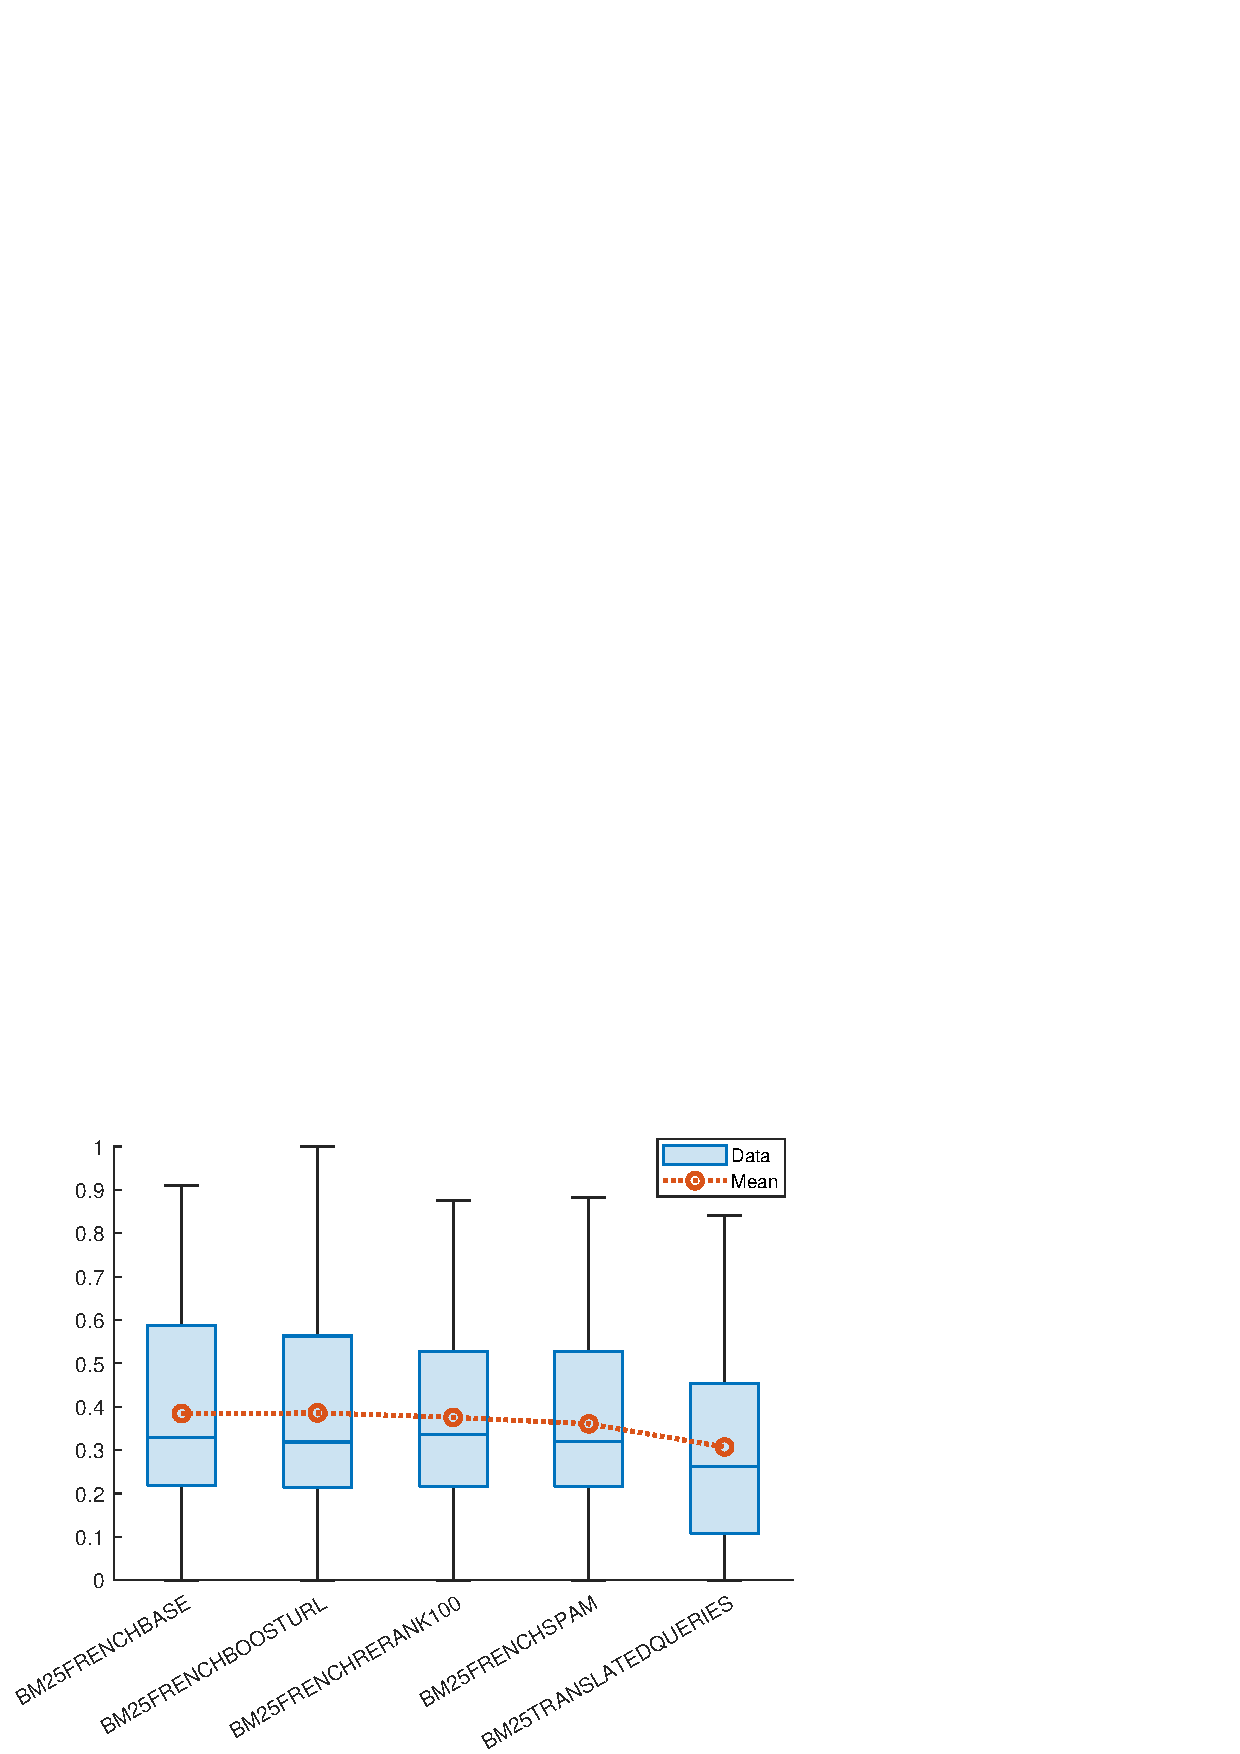
\includegraphics[scale=0.5]{figure/shortterm/boxplot.png}
    \caption{Box Plots Short Term}
    \label{fig:STBP}
\end{figure}
Furthermore we can see that the extension of the whiskers in almost all the systems goes from 0 to 1, this is due to the fact that those systems performs very well for some queries (and reach the maximum value of nDCG) but very poorly for some other queries. A deeper analysis of the results revealed that the queries performing well were very specific while the ones performing badly were either or generic queries or containing terms that can be considered spam (see Section~\ref{subsubsec:spam} for more details).
\par
The two-way \ac{ANOVA} (whose results are reported in Table~\ref{tab:STANOVA}) does reveal relevant differences among the systems since the P-Value result to be lower than the considered threshold. Furthermore, the results of \ac{ANOVA} can be considered reliable since the system contribution is much higher than the error contribution.
\begin{table}[tb]
  \caption{Two-Way ANOVA Short Time}
  \label{tab:STANOVA}
  \centering
  \begin{tabular}{|l|l|l|l|l|l|}
    \toprule
    Source & SS & df & MS & F & prob>F\\
    \midrule
    Columns (systems) & 4.4582 & 4 & 1.1145 & 87.3582 & 7.1783e-71\\
    Rows (topics) & 231.3659 & 881 & 0.2626 & 20.5839 & 0\\
    Error & 44.9605 & 3524 & 0.0128 &  & \\
    Total & 280.7846 & 4409 &  &  & \\
  \bottomrule
\end{tabular}
\end{table}
\par
By looking at the Tukey HSD results (reported in Figure~\ref{fig:sthsd}) we noticed that there is a clear difference between \textit{BM25TRANSLATEDQUERIES} and the other systems, this is due to the fact that this system is based on the English collection. Taken the best system's test (\textit{BM25FRENCHBASE}'s), we see that the \textit{BM25FRENCHBASE} system is significantly different from all systems other than the \textit{BM25FRENCHBOOSTURL} system, this happens because they are basically the same except that the \textit{BM25FRENCHBOOSTURL} system uses an additional field: the URL.
\begin{figure}[tb]
     \centering
     \begin{subfigure}[b]{0.49\textwidth}
         \centering
         \includegraphics[width=\textwidth]{figure/shortterm/tukeyhsd-1.png}
         \caption{BM25FRENCHBASE}
         \label{fig:sthsd1}
     \end{subfigure}
     \hfill
     \begin{subfigure}[b]{0.49\textwidth}
         \centering
         \includegraphics[width=\textwidth]{figure/shortterm/tukeyhsd-2.png}
         \caption{BM25FRENCHBOOSTURL}
         \label{fig:sthsd2}
     \end{subfigure}
     \hfill
     \begin{subfigure}[b]{0.49\textwidth}
         \centering
         \includegraphics[width=\textwidth]{figure/shortterm/tukeyhsd-3.png}
         \caption{BM25FRENCHRERANK100}
         \label{fig:sthsd3}
     \end{subfigure}
     \begin{subfigure}[b]{0.49\textwidth}
         \centering
         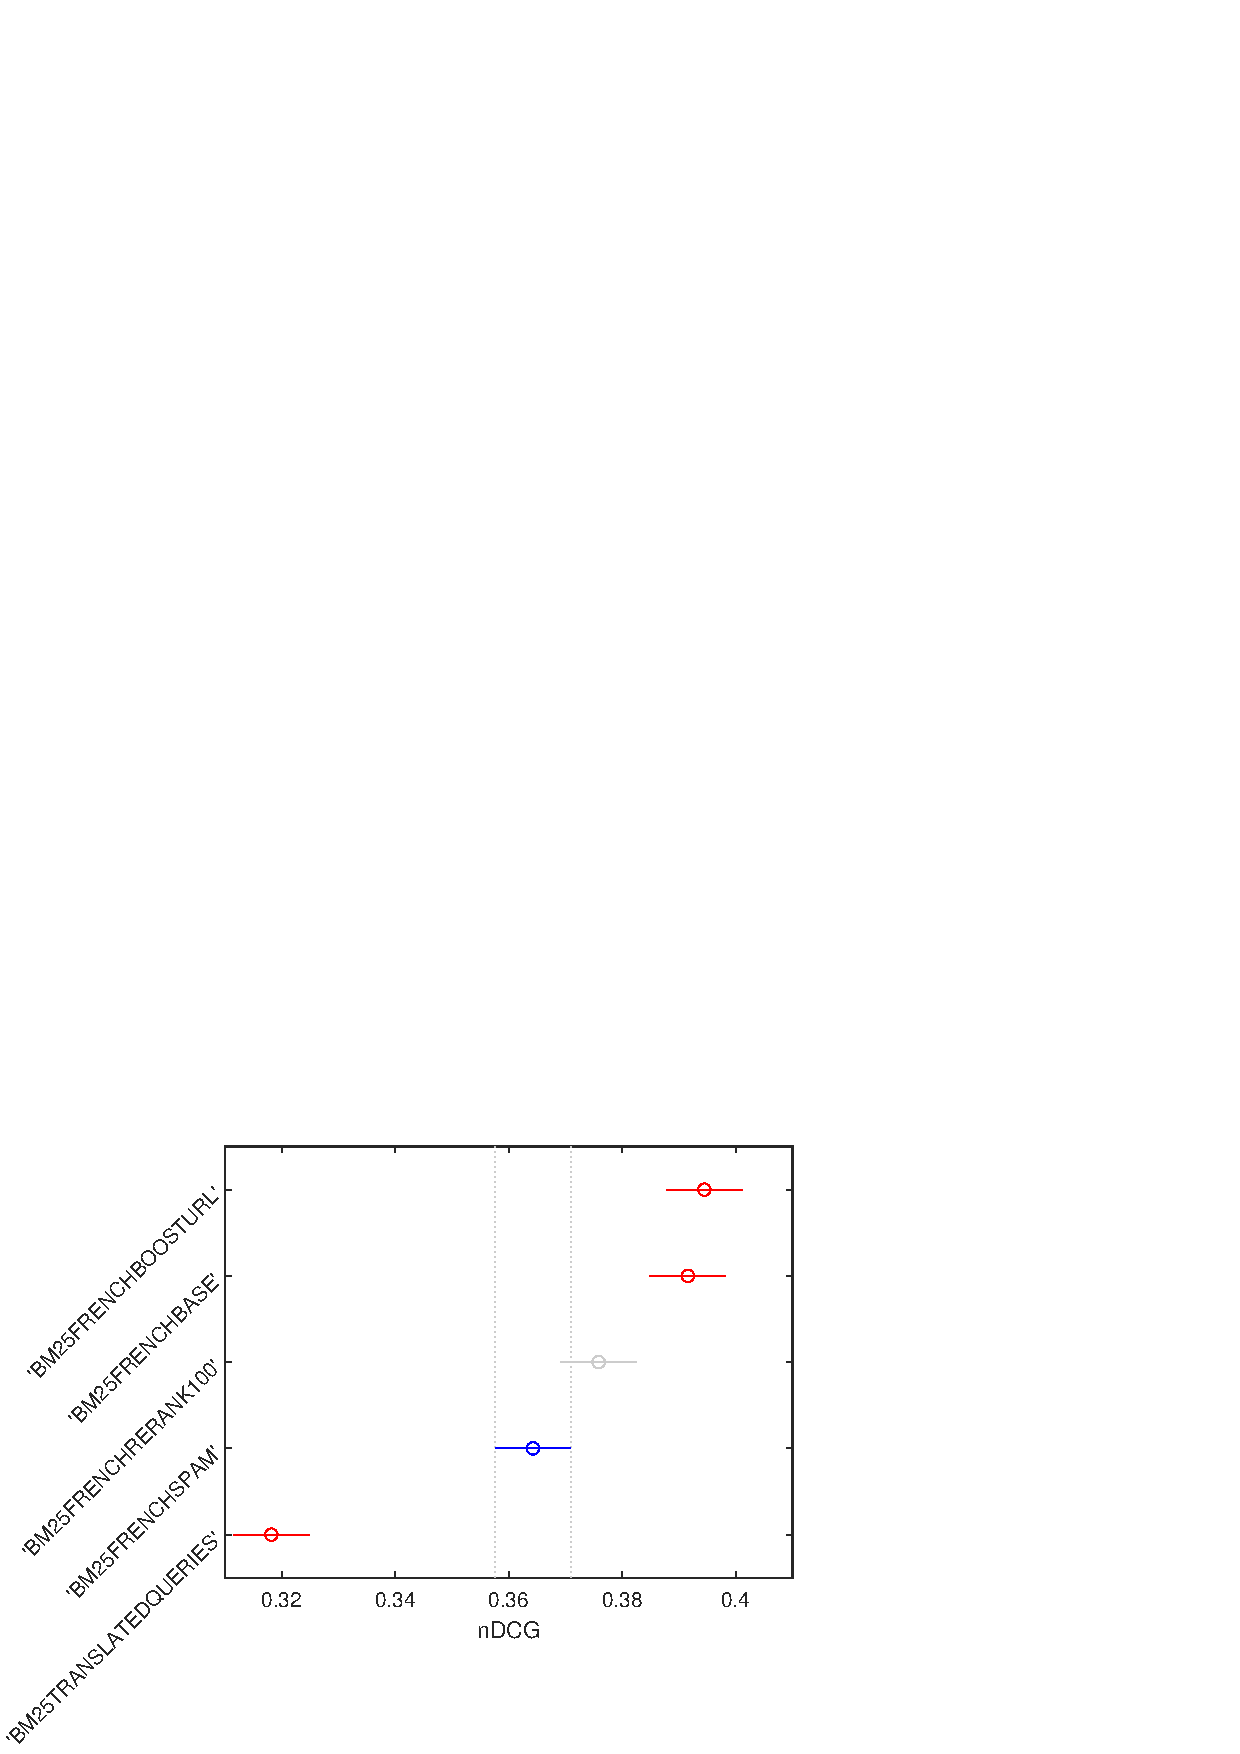
\includegraphics[width=\textwidth]{figure/shortterm/tukeyhsd-4.png}
         \caption{BM25FRENCHSPAM}
         \label{fig:sthsd4}
     \end{subfigure}
     \begin{subfigure}[b]{0.49\textwidth}
         \centering
         \includegraphics[width=\textwidth]{figure/shortterm/tukeyhsd-5.png}
         \caption{BM25TRANSLATEDQUERIES}
         \label{fig:sthsd5}
     \end{subfigure}
        \caption{Tukey HSD Test Short Term}
        \label{fig:sthsd}
\end{figure}


\subsubsection{Long Term}
\label{subsubsec:lt}
From the Box plots reported in Figure~\ref{fig:LTBP} we can see that the systems, even in this case, appear to be quite similar.
\begin{figure}[tb]
    \centering
    \includegraphics[scale=0.8]{figure/longterm/boxplot.eps}
    \caption{Box Plots Long Term}
    \label{fig:LTBP}
\end{figure}
Furthermore we can see that the extension of the whiskers in almost all the systems goes from 0 to 1, this is due to the fact that those systems performs very well for some queries (and reach the maximum value of nDCG) but very poorly for some other queries. A deeper analysis of the results revealed that the queries performing well were very specific while the ones performing badly were either or generic queries or containing terms that can be considered spam (see Section~\ref{subsubsec:spam} for more details).
\par
The two-way \ac{ANOVA} (whose results are reported in Table~\ref{tab:LTANOVA}) does reveal relevant differences among the systems since the P-Value result to be lower than the considered threshold. Furthermore, the results of \ac{ANOVA} can be considered reliable since the system contribution is much higher than the error contribution.
\begin{table}[tb]
  \caption{Two-Way ANOVA Long Time}
  \label{tab:LTANOVA}
  \centering
  \begin{tabular}{|l|l|l|l|l|l|}
    \toprule
    Source & SS & df & MS & F & prob>F\\
    \midrule
    Columns (systems) & 3.5172 & 4 & 0.8793 & 79.2206 & 1.4254e-64\\
    Rows (topics) & 218.3013 & 992 & 0.2368 & 21.3319 & 0\\
    Error & 40.9342 & 3688 & 0.0111 &  & \\
    Total & 262.7527 & 4614 &  &  & \\
  \bottomrule
\end{tabular}
\end{table}
\par
By looking at the Tukey HSD results (reported in Figure~\ref{fig:lthsd}) we noticed that the two best performing systems (\textit{BM25FRENCHBOOSTURL} and \textit{BM25FRENCHBASE}) happen to be quite similar between each other but different from the other systems; this happens because the \textit{BM25FRENCHBOOSTURL} system is actually the same as the \textit{BM25FRENCHBASE} system except that is uses one additional field: the URL. Furthermore, also the \textit{BM25FRENCHRERANK100} system and the \textit{BM25FRENCHSPAM} turn out to be similar while the \textit{BM25TRANSLATEDQUERIES} system still looks different and (as in the previous case studies) this is due to the fact that this last system is based on the English collection.  
\begin{figure}[p]
     \centering
     \begin{subfigure}[b]{0.49\textwidth}
         \centering
         \includegraphics[width=\textwidth]{figure/longterm/tukeyhsd-1.eps}
         \caption{BM25FRENCHBOOSTURL}
         \label{fig:lthsd1}
     \end{subfigure}
     \hfill
     \begin{subfigure}[b]{0.49\textwidth}
         \centering
         \includegraphics[width=\textwidth]{figure/longterm/tukeyhsd-2.eps}
         \caption{BM25FRENCHBASE}
         \label{fig:lthsd2}
     \end{subfigure}
     \hfill
     \begin{subfigure}[b]{0.49\textwidth}
         \centering
         \includegraphics[width=\textwidth]{figure/longterm/tukeyhsd-3.eps}
         \caption{BM25FRENCHRERANK100}
         \label{fig:lthsd3}
     \end{subfigure}
     \begin{subfigure}[b]{0.49\textwidth}
         \centering
         \includegraphics[width=\textwidth]{figure/longterm/tukeyhsd-4.eps}
         \caption{BM25FRENCHSPAM}
         \label{fig:lthsd4}
     \end{subfigure}
     \begin{subfigure}[b]{0.49\textwidth}
         \centering
         \includegraphics[width=\textwidth]{figure/longterm/tukeyhsd-5.eps}
         \caption{BM25TRANSLATEDQUERIES}
         \label{fig:lthsd5}
     \end{subfigure}
        \caption{Tukey HSD Test Long Term}
        \label{fig:lthsd}
\end{figure}